\documentclass[11pt,a4paper,twoside,dutch]{article}
\usepackage{subcaption}
\usepackage[alsoload=astronomy]{siunitx}
\title{Fysica van Galaxie\"en\\Programmeerproject}
\author{Kevin Canters \\ Alexandro Fulco \\ Frederic Van Assche}
\date{2 juni 2014}

\usepackage[dutch]{babel}
\usepackage{amsmath,amssymb,amsfonts,textcomp}
\usepackage{graphicx,epsfig}
\usepackage{float,flafter}
\usepackage{hyperref}
\usepackage{inputenc}
\usepackage{multicol}
\usepackage{lastpage}
\usepackage{fancyhdr}
\usepackage[hypcap]{caption}
\usepackage{sectsty}
\usepackage{enumitem}
\usepackage{dcolumn}
\usepackage{siunitx}
\usepackage{booktabs}
\usepackage{graphicx}
\usepackage{threeparttable}
\usepackage{textcomp}
\usepackage{gensymb}
\usepackage[table]{xcolor}
\usepackage{varioref}
\usepackage[plain]{fancyref}
\usepackage{subfiles}

\setlength\paperwidth{20.999cm}
\setlength\paperheight{29.699cm}
\setlength\voffset{-1in}
\setlength\hoffset{-1in}
\setlength\topmargin{1.499cm}
\setlength\headheight{14pt}
\setlength\headsep{1cm}
\setlength\footskip{1.131cm}
\setlength\textheight{25cm}
\setlength\oddsidemargin{2.499cm}
\setlength\textwidth{15.999cm}

\captionsetup{font={normalsize},labelfont={bf}}

\sectionfont{\sectionrule{0pt}{0pt}{-5pt}{0.8pt}}

\numberwithin{equation}{section}
%\numberwithin{figure}{section}
%\numberwithin{table}{section}

\newcommand{\ra}[1]{\renewcommand{\arraystretch}{#1}}

\ra{1.3}
\setlength{\tabcolsep}{12pt}

\newenvironment{Figure}
  {\par\medskip\noindent\minipage{\linewidth}}
  {\endminipage\par\medskip}

\newcommand{\AF}{\mathop{\mathrm{AF}}}
\newcommand{\RF}{\mathop{\mathrm{RF}}}
\newcommand{\SF}{\mathop{\mathrm{SF}}}

\newcommand{\insertgraph}[3]{\begin{figure}[h]
\centering
\captionsetup{type=figure}
\input{graph/#1}
\captionof{figure}{#2}
\label{#3}
\end{figure}}

\newcommand{\inserttable}[3]{\begin{table}[h]
\input{table/#1}
\caption{#2}
\label{#3}
\end{table}}

\newcommand{\insertfigure}[5]{\begin{figure}[h]
\centering
\includegraphics[#5]{img/#1.jpg}
\caption{#2}
~ \\
\emph{Bron: #3}
\label{#4}
\end{figure}}

\newcommand{\insertFigure}[4]{\begin{Figure}
\centering
\captionsetup{type=figure}
\includegraphics[#4]{img/#1.jpg}
\captionof{figure}{#2}
\label{#3}
\end{Figure}}

\definecolor{lightgray}{gray}{0.9}

\makeatletter
\usepackage{graphicx}
\begin{document}
\begin{titlepage}
	\vspace*{\fill}
	\begin{center}
		{\bf {\Huge \@title}} \\
		\vspace{.5cm}
		{\bf {\large \sc \@author}} \\

		\vspace{.4cm}

		\vspace{.8cm}
		Academiejaar 2013-2014
		\vspace{1cm}

	\end{center}
	\vspace*{\fill}
\end{titlepage}

\pagestyle{fancy}
%\lhead{\@author}
\lhead{Kevin Canters \& Alexandro Fulco \& Frederic Van Assche}
%\chead{{\sc \@title}}
%\rhead{Academiejaar 2013-2014}
\rhead{}
\lfoot{}
\cfoot{\thepage\ van \pageref{LastPage}}
\rfoot{}
\setcounter{page}{1}
\renewcommand{\footrulewidth}{0.4pt}
\renewcommand{\headrulewidth}{0.4pt}


\section{Uitdrukking voor dichtheid}
Voor de triaxiale zwaartekrachtpotentiaal geldt dat
$$V(x,y,z) = \dfrac{v_0^2}{2}\ln \left( 1 + x^2 + \dfrac{y^2}{a^2} + \dfrac{z^2}{b^2}\right)$$
Om hieruit de dichtheid $\rho(x,y,z)$ te halen die hiermee overeenstemt, maken we gebruik van de vergelijking van Poisson voor de zwaartekracht
$$\nabla^2 \phi(x,y,z) = 4 \pi G \rho(x,y,z)$$
In dit geval geldt dat $\phi(x,y,z) = V(x,y,z)$. De uitdrukking voor $\rho(x,y,z)$ hebben we via Python met symbolische differentiatie bekomen, en is
$$4 \pi G \rho(x,y,z) = \dfrac{-(v_0^2 (a^4 (b^4 (x^2-1)-b^2 (x^2+z^2+1)+z^2)-a^2 b^2 (b^2 (x^2+y^2+1)+y^2+z^2)+b^4 y^2))}{(a^2 (b^2 (x^2+1)+z^2)+b^2 y^2)^2}$$
Met deze uitdrukking hebben we ter illustratie en controle in figuur~\ref{fig:mass} een plot gemaakt die de massaverdeling binnen de galaxie weergeeft.
\\

Als we nu willen weten aan welke voorwaarde $b$ moet voldoen, met $1 > a > b$, opdat de dichtheid overal positief is, kunnen we dit probleem schrijven als een set van vergelijking (ofwel, in matrixvorm). De noemer is altijd positief, dus deze kunnen we uit het probleem halen. $v_0^2$ kunnen we ook uit het probleem halen, omwille van dezelfde reden. De voorfactor $(4\pi G)^{-1}$ kunnen we daarom dus ook laten vallen. Het resultaat, in matrixvorm, is dan

\begin{equation*}\left(
\begin{array}{cccc}
 0 & a^2 b^4-b^4+a^2 b^2 & b^2 a^4-a^4+b^2 a^2 & b^4 a^4+b^2 a^4+b^4 a^2 \\
 -b^4 a^4+b^2 a^4+b^4 a^2 & 0 & b^2 a^4-a^4+b^2 a^2 & b^4 a^4+b^2 a^4+b^4 a^2 \\
 -b^4 a^4+b^2 a^4+b^4 a^2 & a^2 b^4-b^4+a^2 b^2 & 0 & b^4 a^4+b^2 a^4+b^4 a^2 \\
 0 & 0 & 0 & b^4 a^4+b^2 a^4+b^4 a^2 \\
\end{array}
\right)
\end{equation*}
De determinant van deze matrix is
\begin{align*}
D &= a^2 b^2 \left(a^4 b^4+a^4 b^2+a^2 b^4\right) \times \nonumber \\& \left(-2 a^8 b^8+2 a^8 b^6+2 a^8 b^4-2 a^8 b^2+2 a^6 b^8-4 a^6 b^6+2 a^6 b^4+2 a^4 b^8+2 a^4 b^6-2 a^2 b^8\right)
\end{align*}
Als oplossingen vinden we, met alle (8) mogelijke permutaties van de tekens
$$b > \pm \frac{a}{\sqrt{\pm a^2 \pm 1}}$$
Echter, de enige fysisch relevante oplossing is die waarbij $b > 0$, en de wortel nergens singulier is
$$b > \frac{a}{\sqrt{a^2 + 1}}$$

\pagebreak
\section{Eenheden}
De gebruikte eenheden staan in onderstaande tabel~\ref{tab:eenheden} weergegeven. Als constante $G$ gebruikten we $G = \SI{4.302e-6}{\kilo\parsec\kilo\meter\squared\per\second\squared}M_\odot^{-1}$.
\\

\begin{table}[h]
\centering
\begin{tabular}{lcl}
	\hline
	\textbf{Grootheid} & \textbf{Symbool} & \textbf{Eenheid} \\
	\hline
	Afstanden & $x$ & \si{\kilo\parsec}\\
	Snelheden & $v$ & \si{\kilo\meter\per\second}\\
	Massa's & $m$ & M$_{\odot}$ \\
	Tijden & $t$ & \si{\second\kilo\meter\per\parsec} $\approx$ \num{950e6}yr\\
	\hline
\end{tabular}
\caption{Gebruikte eenheden}
\label{tab:eenheden}
\end{table}


\section{Voorbeeldbanen}

De drie types banen werden gesimuleerd en geplot:
\begin{enumerate}
\item \textbf{Box orbits}\\
De parameters staan opgelijst in tabel~\ref{tab:boxparam}, en de bekomen baan is weergegeven in figuur~\ref{fig:boxplot}.
\item \textbf{Long axis tube}\\
De parameters staan opgelijst in tabel~\ref{tab:longparam}, en de bekomen baan is weergegeven in figuur~\ref{fig:longplot}.
\item \textbf{Short axis tube}\\
De parameters staan opgelijst in tabel~\ref{tab:shortparam}, en de bekomen baan is weergegeven in figuur~\ref{fig:shortplot}.
\end{enumerate}

De doorsnijdingen met het oppervlak van constante energie $E = V(x,y,z)$ zijn weergegeven in dikke zwarte contouren op de verschillende grafieken.

\section{Effect van zwart gat}
Tenslotte hebben we een puntpotentiaal van een zwart gat toegevoegd aan het model. We lieten $M_\bullet$ vari\"eren van \num{3.1e7} M$_\odot$ tot \num{10e8} M$_\odot$ in zes stappen (telkens verdubbeling van $M_\bullet$. Het resultaat werd geplot in figuur~\ref{fig:bhplot}. Als baan werd dezelfde gebruikt als voor de box orbit, weergegeven in tabel~\ref{tab:boxparam}.

Het effect van de extra puntpotentiaal van het zwart gat manifesteerde zich bij kleine $M_\bullet$ als een kleine perturbatie van de baan. Bij stijgende massa keren de rollen van de galactische potentiaal als geperturbeerde en $M_\bullet$-potentiaal als perturbatie geleidelijk om. Bij grote $M_\bullet$ begint het zwart gat uiteindelijk de gehele potentiaal te overheersen en gaan we over van een triaxiaal systeem richting een eerder sferisch symmetrisch systeem. In dit systeem worden de sterbanen zeer chaotisch, en beginnen ze het hele oppervlak van constante energie op te vullen.

Deze neiging naar sferische symmetrie hebben we nog eens geverifieerd door een plot te maken met $M_\bullet = 10^{10}$~M$_{\odot}$, weergegeven in figuur~\ref{fig:bigbhplot}. Voor deze plot werden ook dezelfde parameters gebruikt als in tabel~\ref{tab:boxparam}. In deze figuur zien we inderdaad dat de galaxie zijn triaxialiteit verliest wanneer het zwart gat aan massa wint.

\newpage
\begin{figure}[b]
\centering
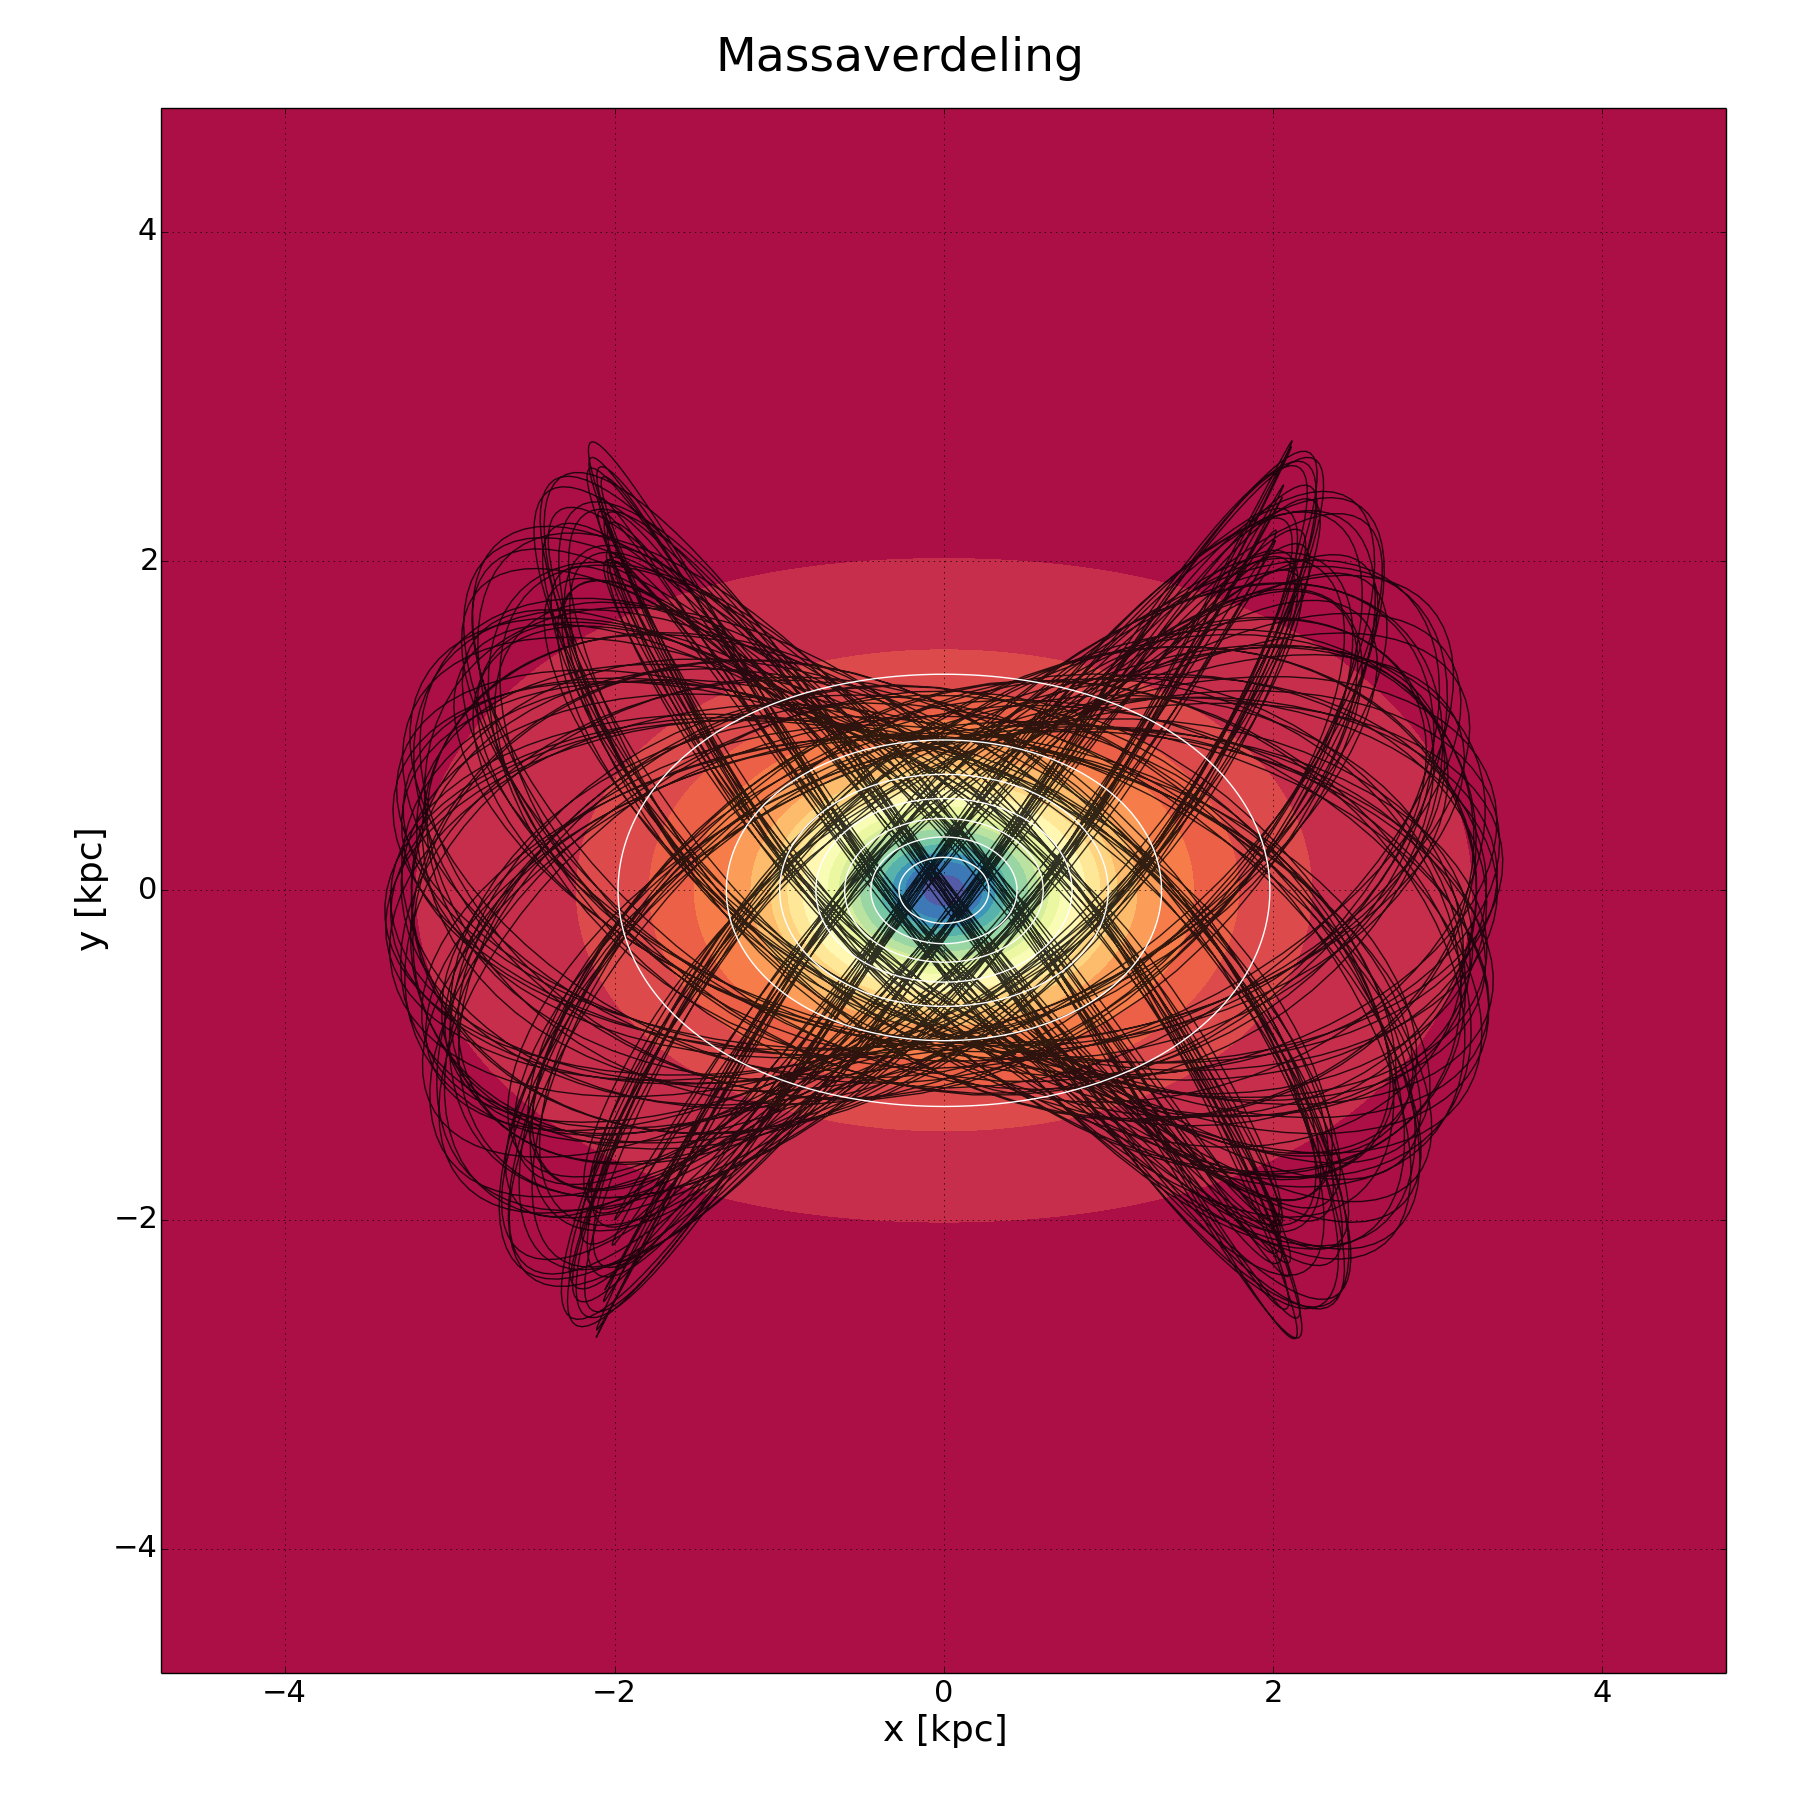
\includegraphics[width=1\textwidth]{img/mass.png}
\caption{Massaverdeling}
\label{fig:mass}
\end{figure}

\begin{table}[t]
\centering
\begin{tabular}{lcr}
	\hline
	\textbf{Parameter} & \textbf{Symbool} & \textbf{Waarde} \\
	\hline
	Lange as & $a$ & $0.8$\\
	Korte as & $b$ & $0.75$\\
	Galactische circkelsnelheid & $v_c$ & \SI{220}{\kilo\meter\per\second}\\
	Beginpositie & $\vec{x_0}$ & (2, 2, 2)~\si{\kilo\parsec}\\
	Beginsnelheid & $\vec{v_0}$ & (0, 0, 0)~\si{\kilo\meter\per\second}\\
	Integratietijd & $T$ & \SI{10}{\second\kilo\meter\per\parsec} $\approx$ \num{9.5e9}~yr \\
	\hline
\end{tabular}
\caption{Parameters voor box orbit in massaverdelingsplot}
\label{tab:massparam}
\end{table}

\newpage

\begin{figure}[b]
\centering
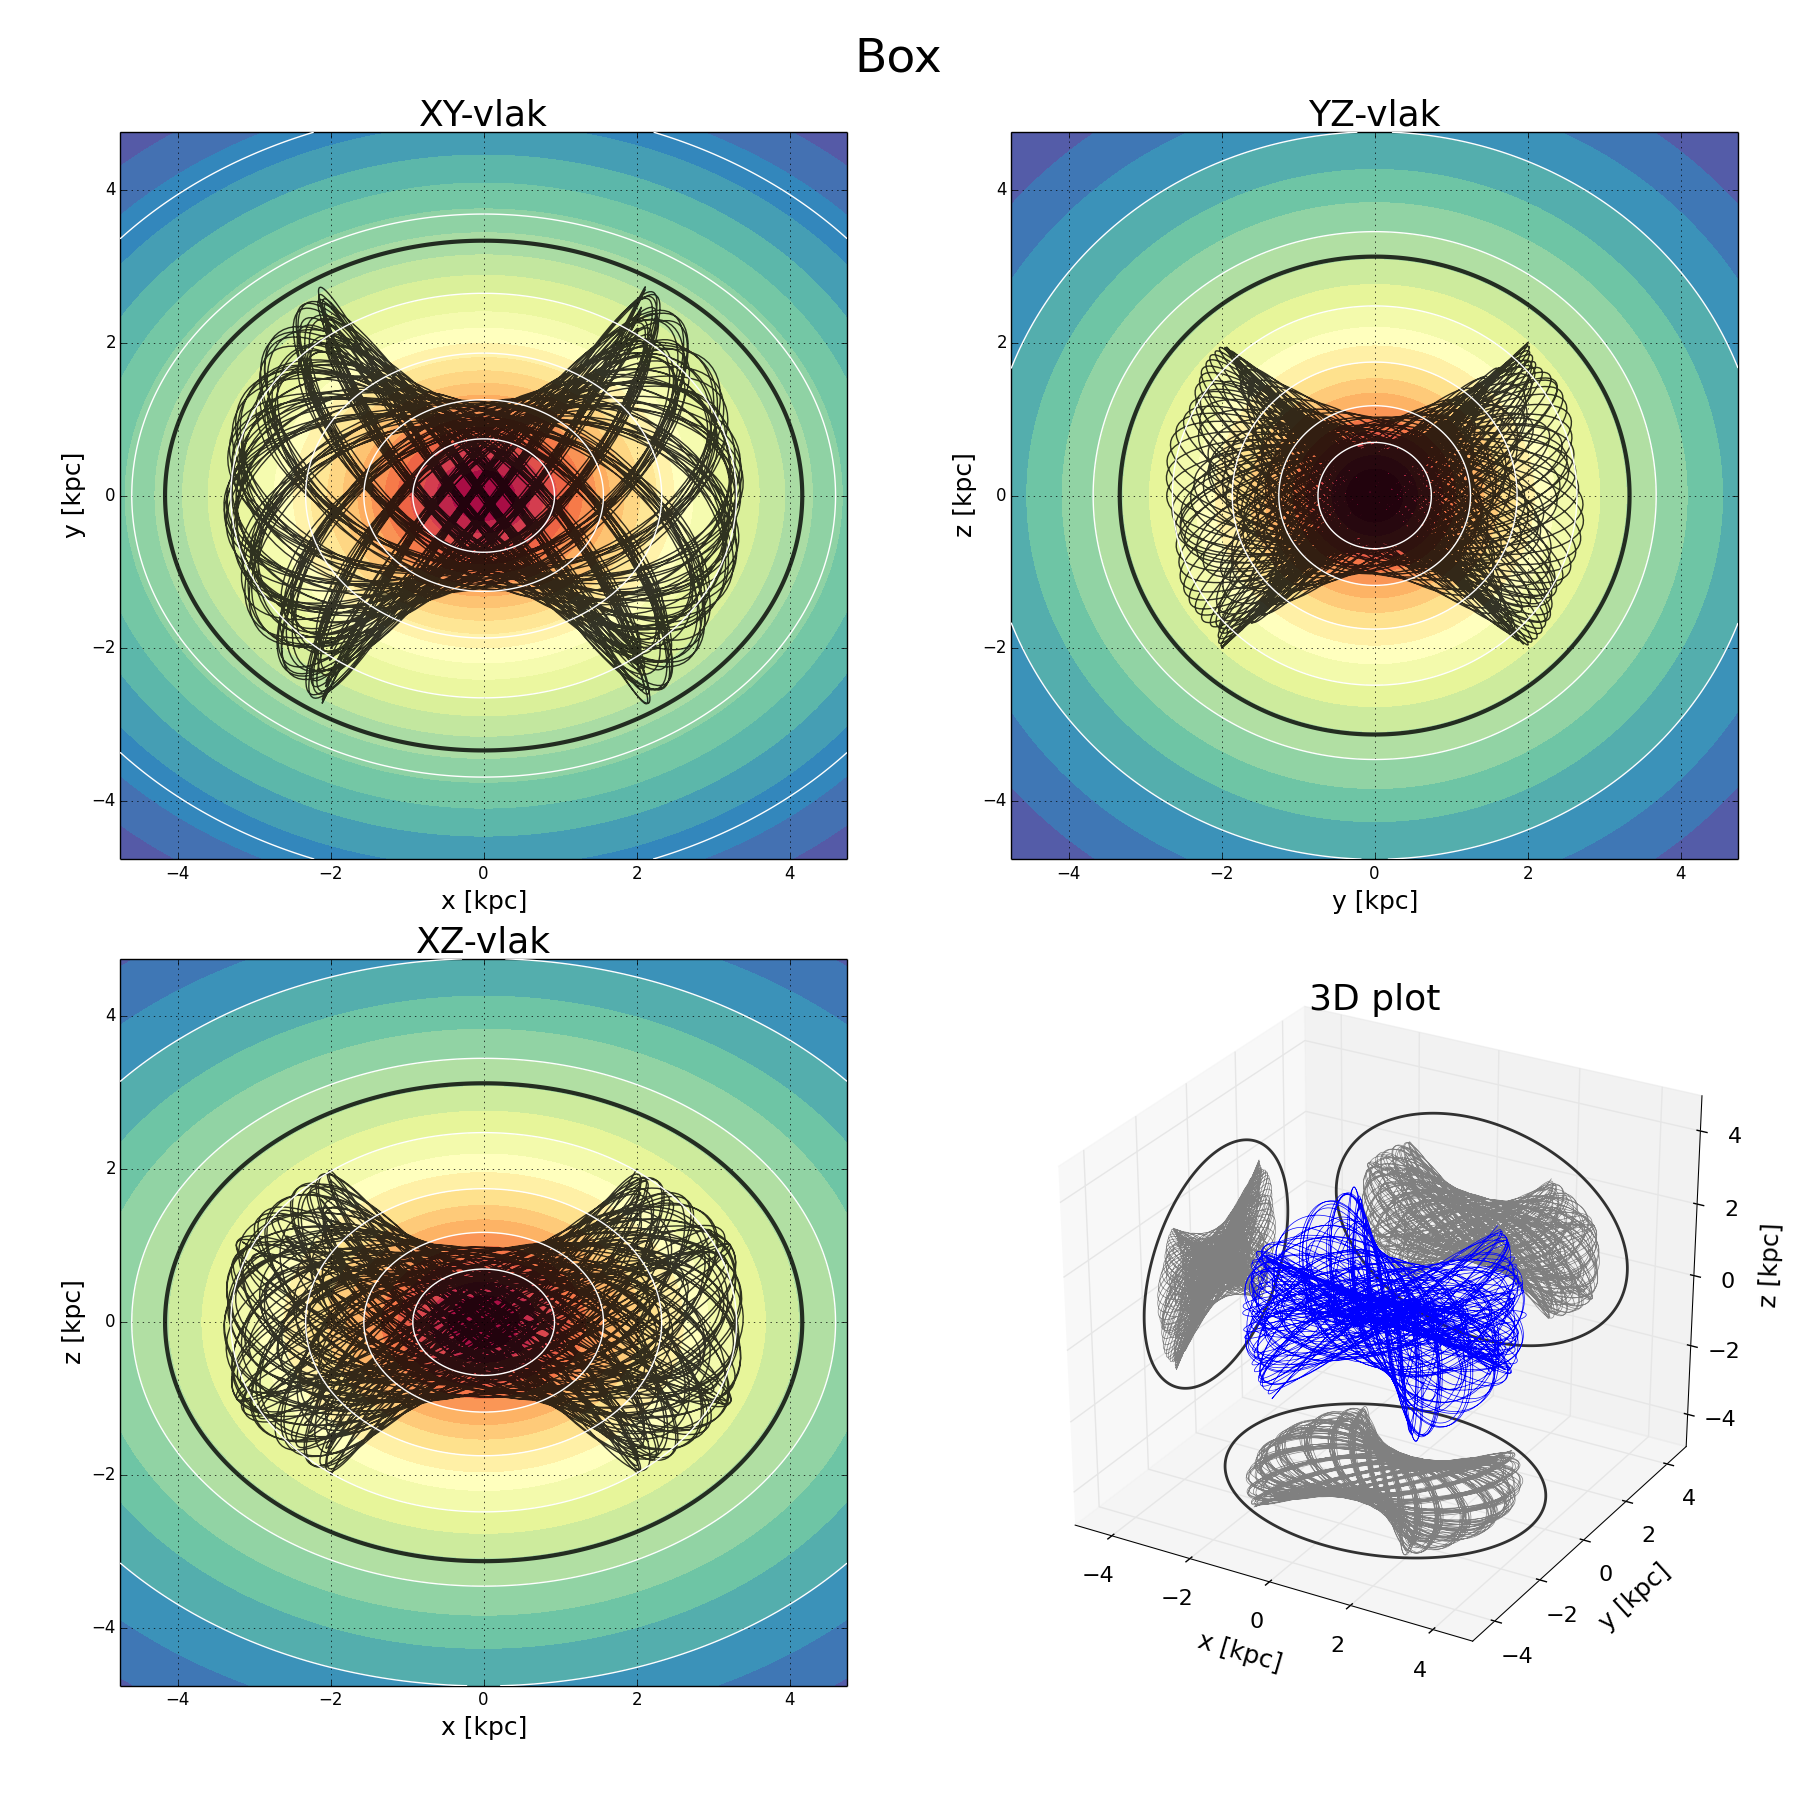
\includegraphics[width=1\textwidth]{img/box.png}
\caption{Box orbit}
\label{fig:boxplot}
\end{figure}

\begin{table}[t]
\centering
\begin{tabular}{lcr}
	\hline
	\textbf{Parameter} & \textbf{Symbool} & \textbf{Waarde} \\
	\hline
	Lange as & $a$ & $0.8$\\
	Korte as & $b$ & $0.75$\\
	Galactische circkelsnelheid & $v_c$ & \SI{220}{\kilo\meter\per\second}\\
	Beginpositie & $\vec{x_0}$ & (2, 2, 2)~\si{\kilo\parsec}\\
	Beginsnelheid & $\vec{v_0}$ & (0, 0, 0)~\si{\kilo\meter\per\second}\\
	Integratietijd & $T$ & \SI{10}{\second\kilo\meter\per\parsec} $\approx$ \num{9.5e9}~yr \\
	\hline
\end{tabular}
\caption{Parameters voor box orbit}
\label{tab:boxparam}
\end{table}

\newpage
\begin{figure}[t]
\centering
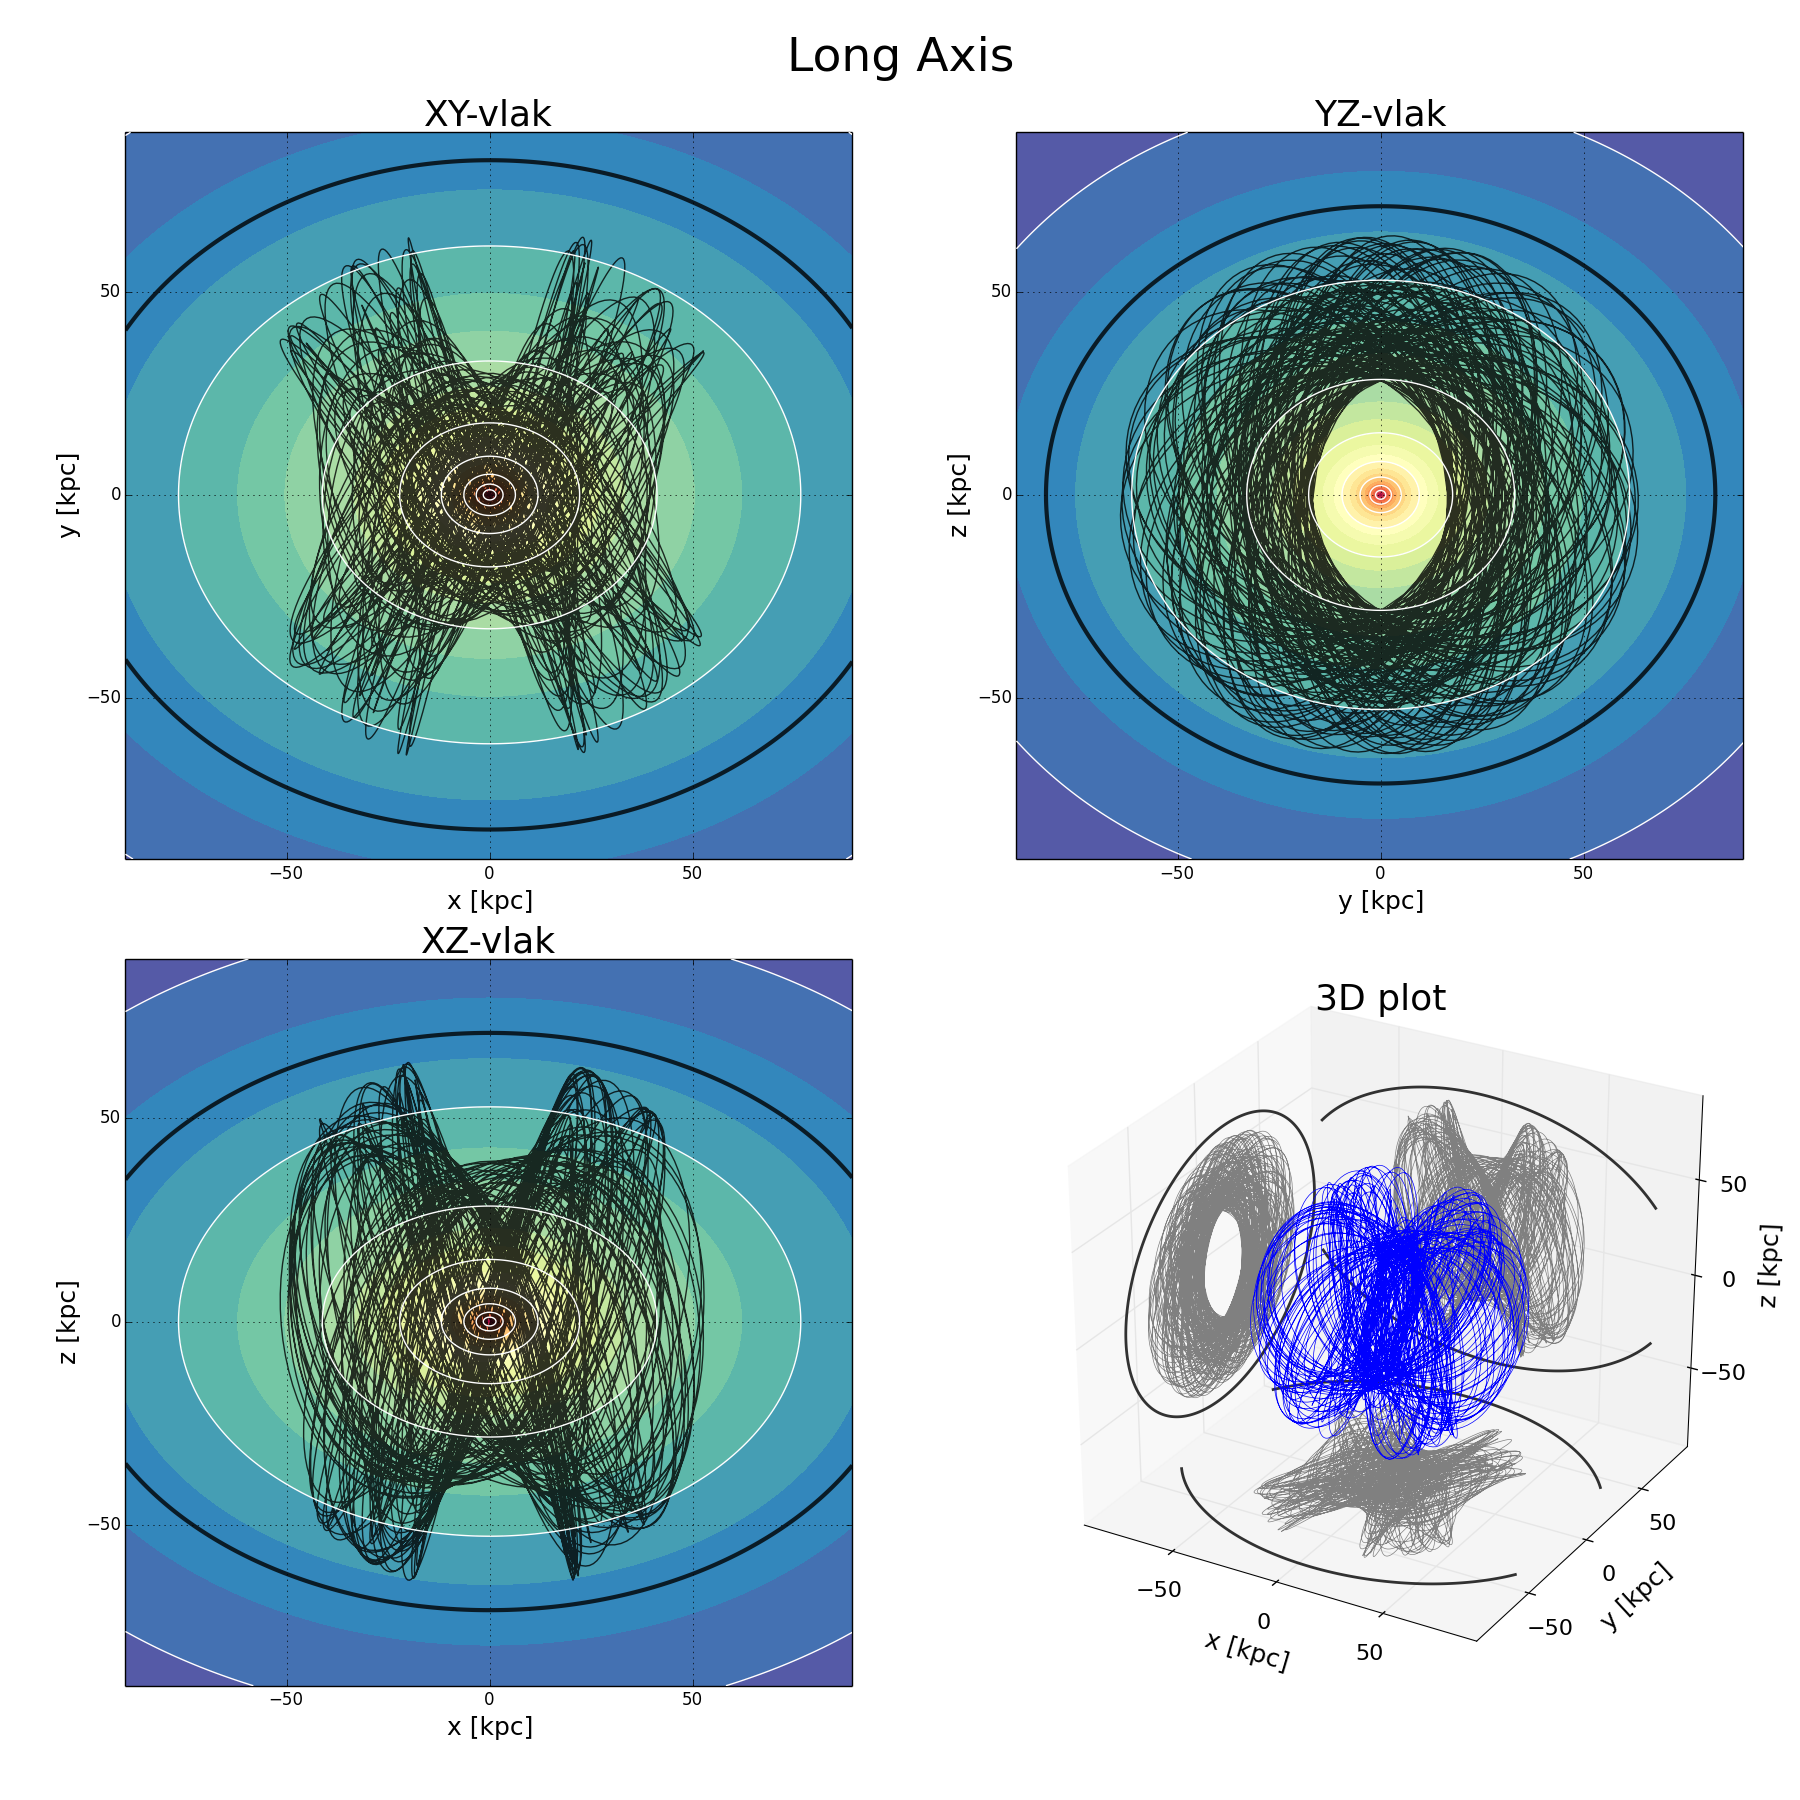
\includegraphics[width=1\textwidth]{img/long.png}
\caption{Long axis tube}
\label{fig:longplot}
\end{figure}

\begin{table}[b]
\centering
\begin{tabular}{lcr}
	\hline
	\textbf{Parameter} & \textbf{Symbool} & \textbf{Waarde} \\
	\hline
	Lange as & $a$ & $0.8$\\
	Korte as & $b$ & $0.69$\\
	Galactische circkelsnelheid & $v_c$ & \SI{220}{\kilo\meter\per\second}\\
	Beginpositie & $\vec{x_0}$ & (20, 50, 40)~\si{\kilo\parsec}\\
	Beginsnelheid & $\vec{v_0}$ & (10, -75, 100)~\si{\kilo\meter\per\second}\\
	Integratietijd & $T$ & \SI{200}{\second\kilo\meter\per\parsec} $\approx$ \num{1.9e11}~yr \\
	\hline
\end{tabular}
\caption{Parameters voor long axis tube}
\label{tab:longparam}
\end{table}

\newpage
\begin{figure}[t]
\centering
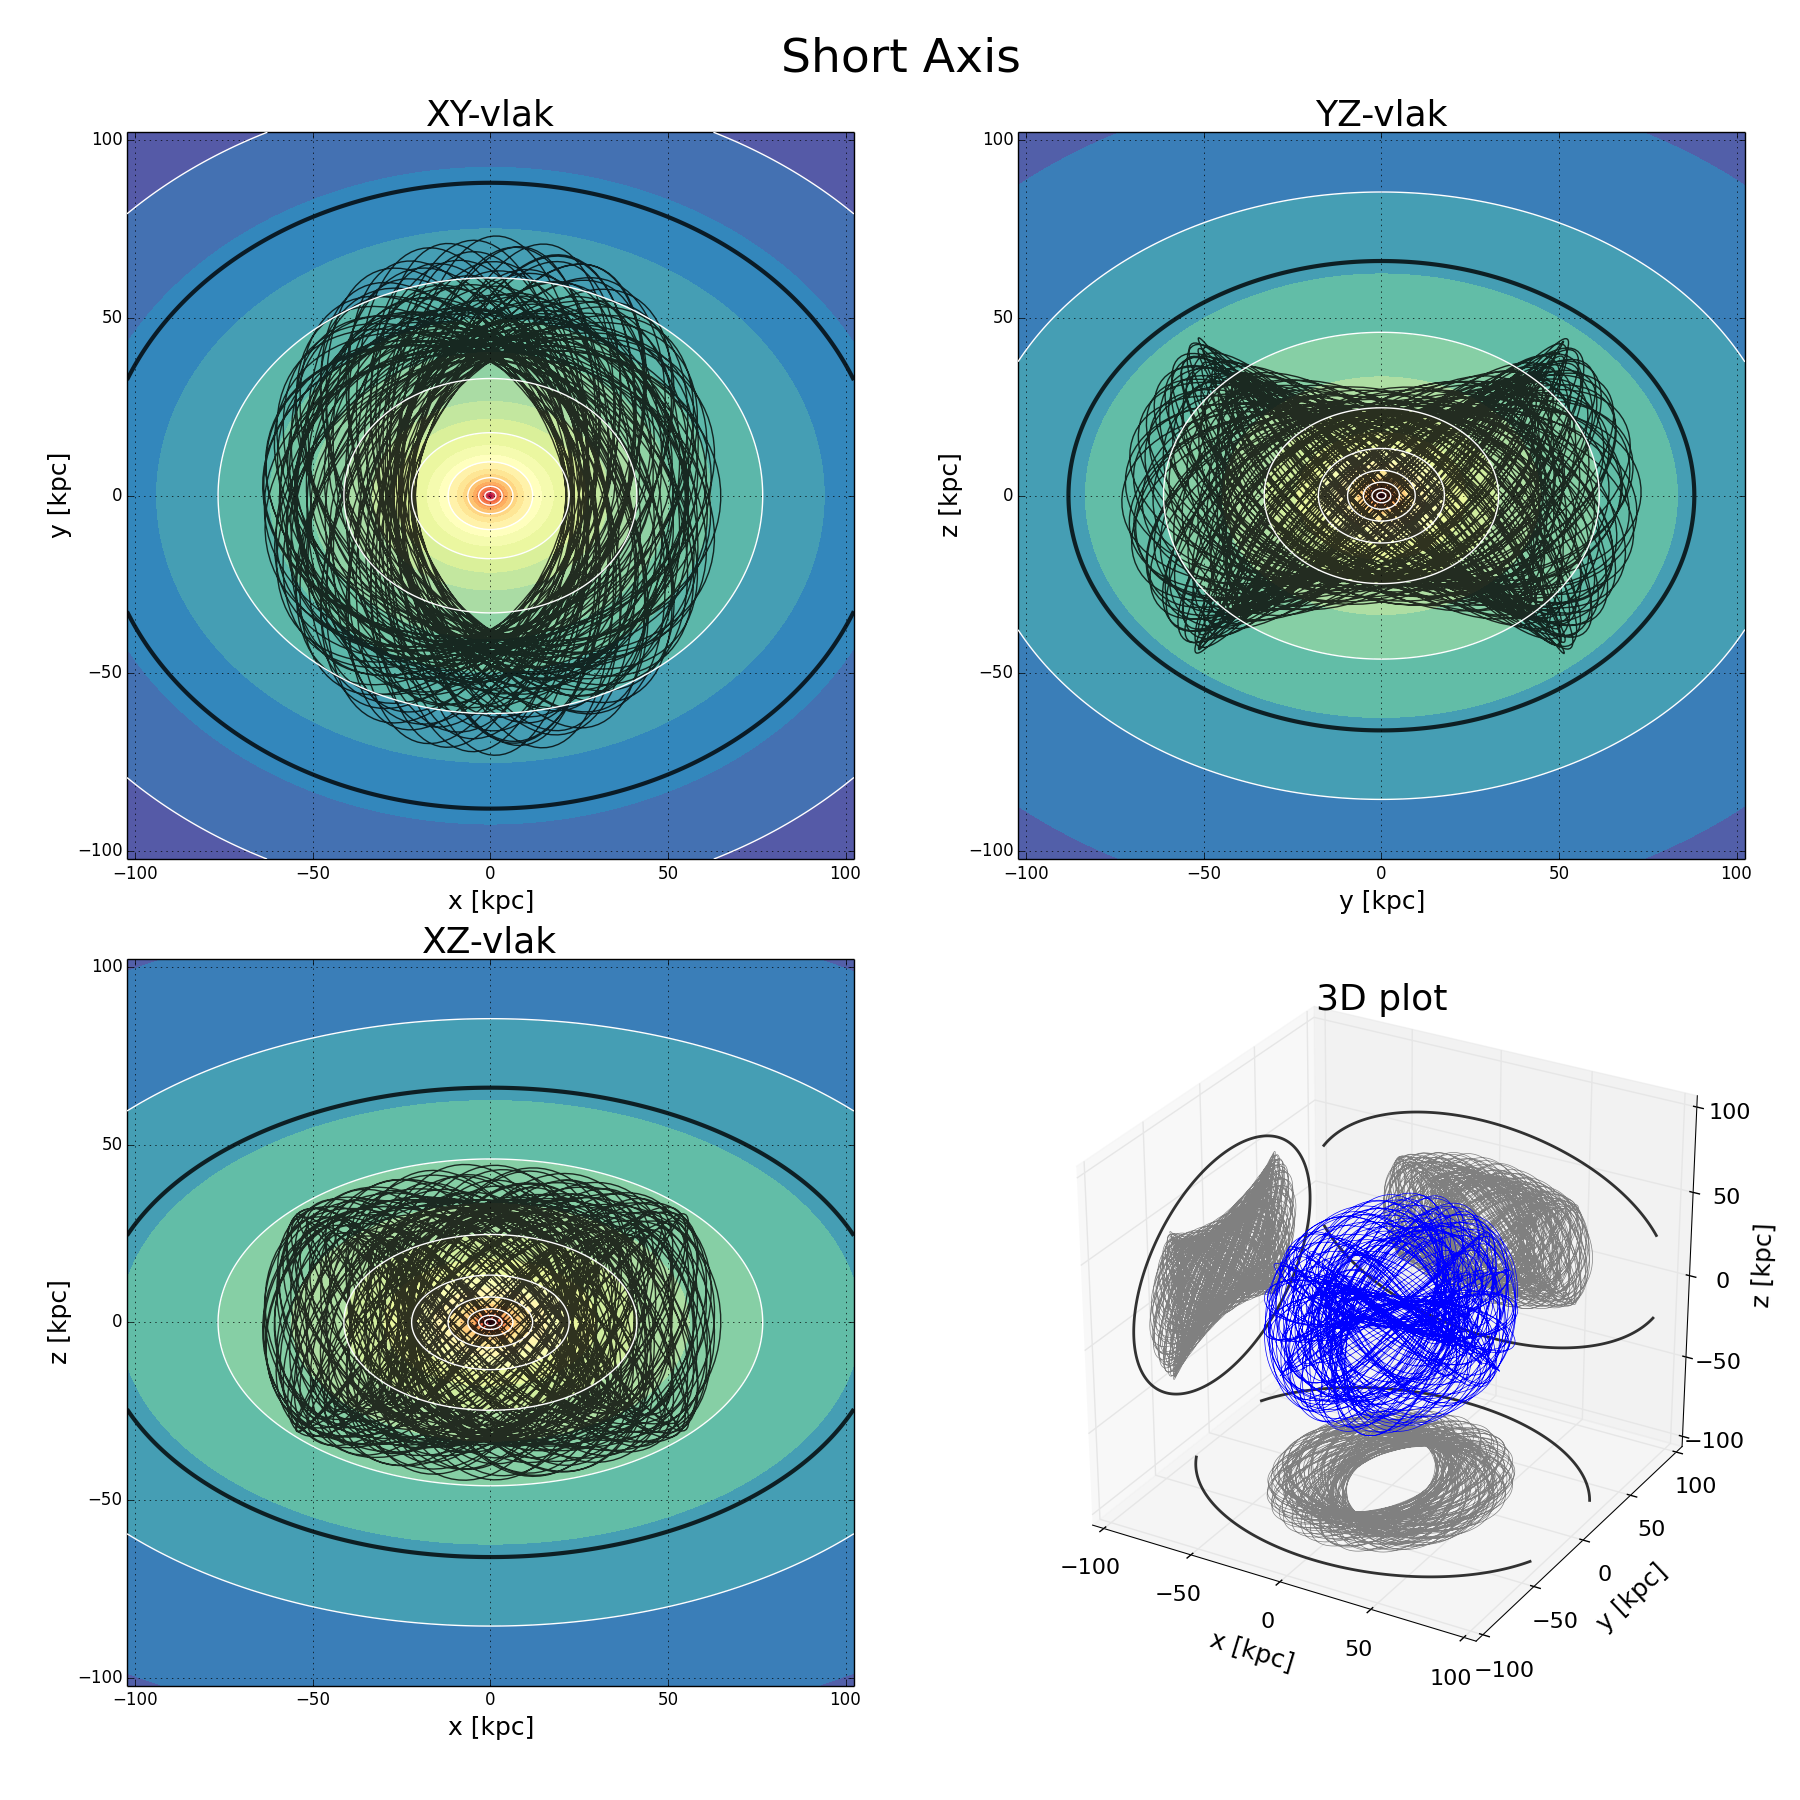
\includegraphics[width=1\textwidth]{img/short.png}
\caption{Short axis tube}
\label{fig:shortplot}
\end{figure}

\begin{table}[b]
\centering
\begin{tabular}{lcr}
	\hline
	\textbf{Parameter} & \textbf{Symbool} & \textbf{Waarde} \\
	\hline
	Lange as & $a$ & $0.8$\\
	Korte as & $b$ & $0.6$\\
	Galactische circkelsnelheid & $v_c$ & \SI{220}{\kilo\meter\per\second}\\
	Beginpositie & $\vec{x_0}$ & (20, 50, 40)~\si{\kilo\parsec}\\
	Beginsnelheid & $\vec{v_0}$ & (100, -75, 10)~\si{\kilo\meter\per\second}\\
	Integratietijd & $T$ & \SI{200}{\second\kilo\meter\per\parsec} $\approx$ \num{1.9e11}~yr \\
	\hline
\end{tabular}
\caption{Parameters voor short axis tube}
\label{tab:shortparam}
\end{table}

\newpage
\vfill
\begin{figure}
\centering
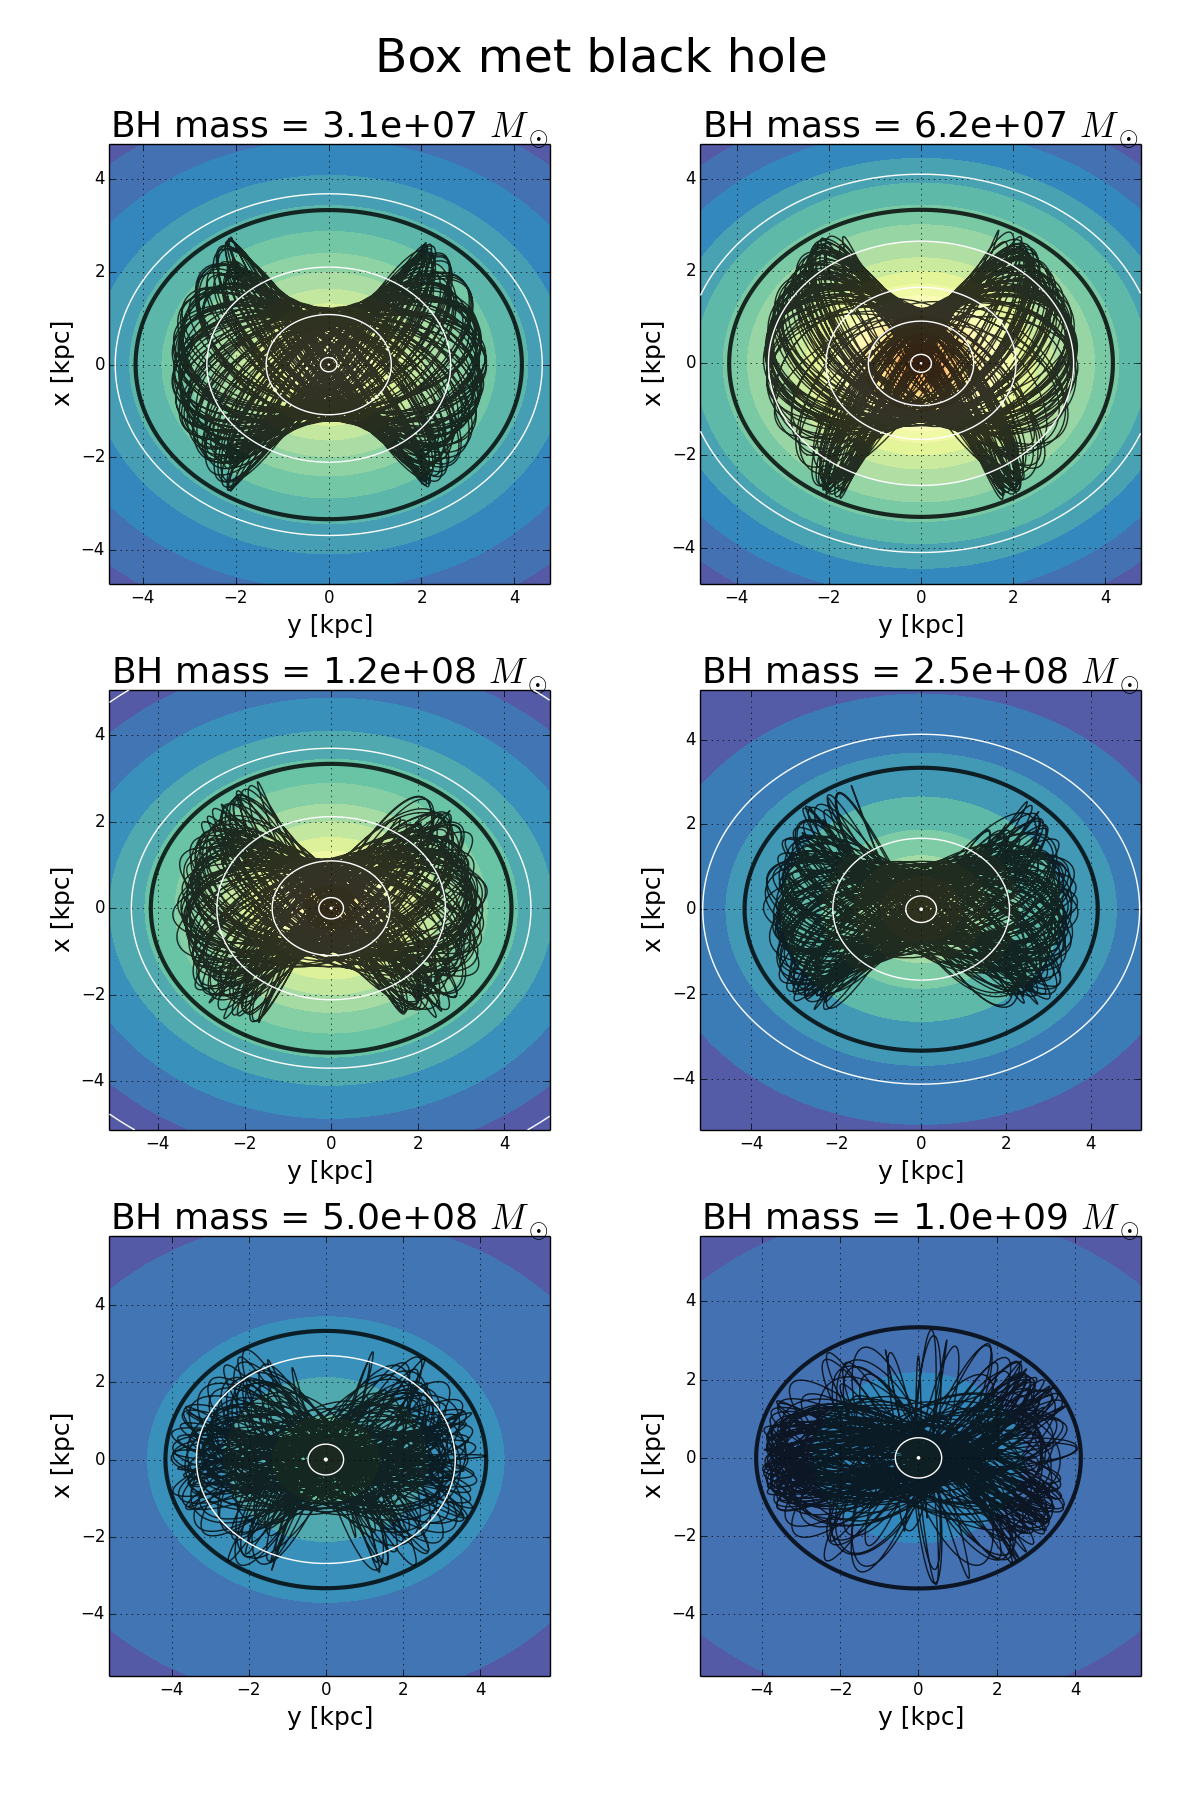
\includegraphics[width=1\textwidth]{img/box_bh.png}
\caption{Effect van een zwart gat}
\label{fig:bhplot}
\end{figure}
\vfill

\newpage
\vfill
\begin{figure}
\centering
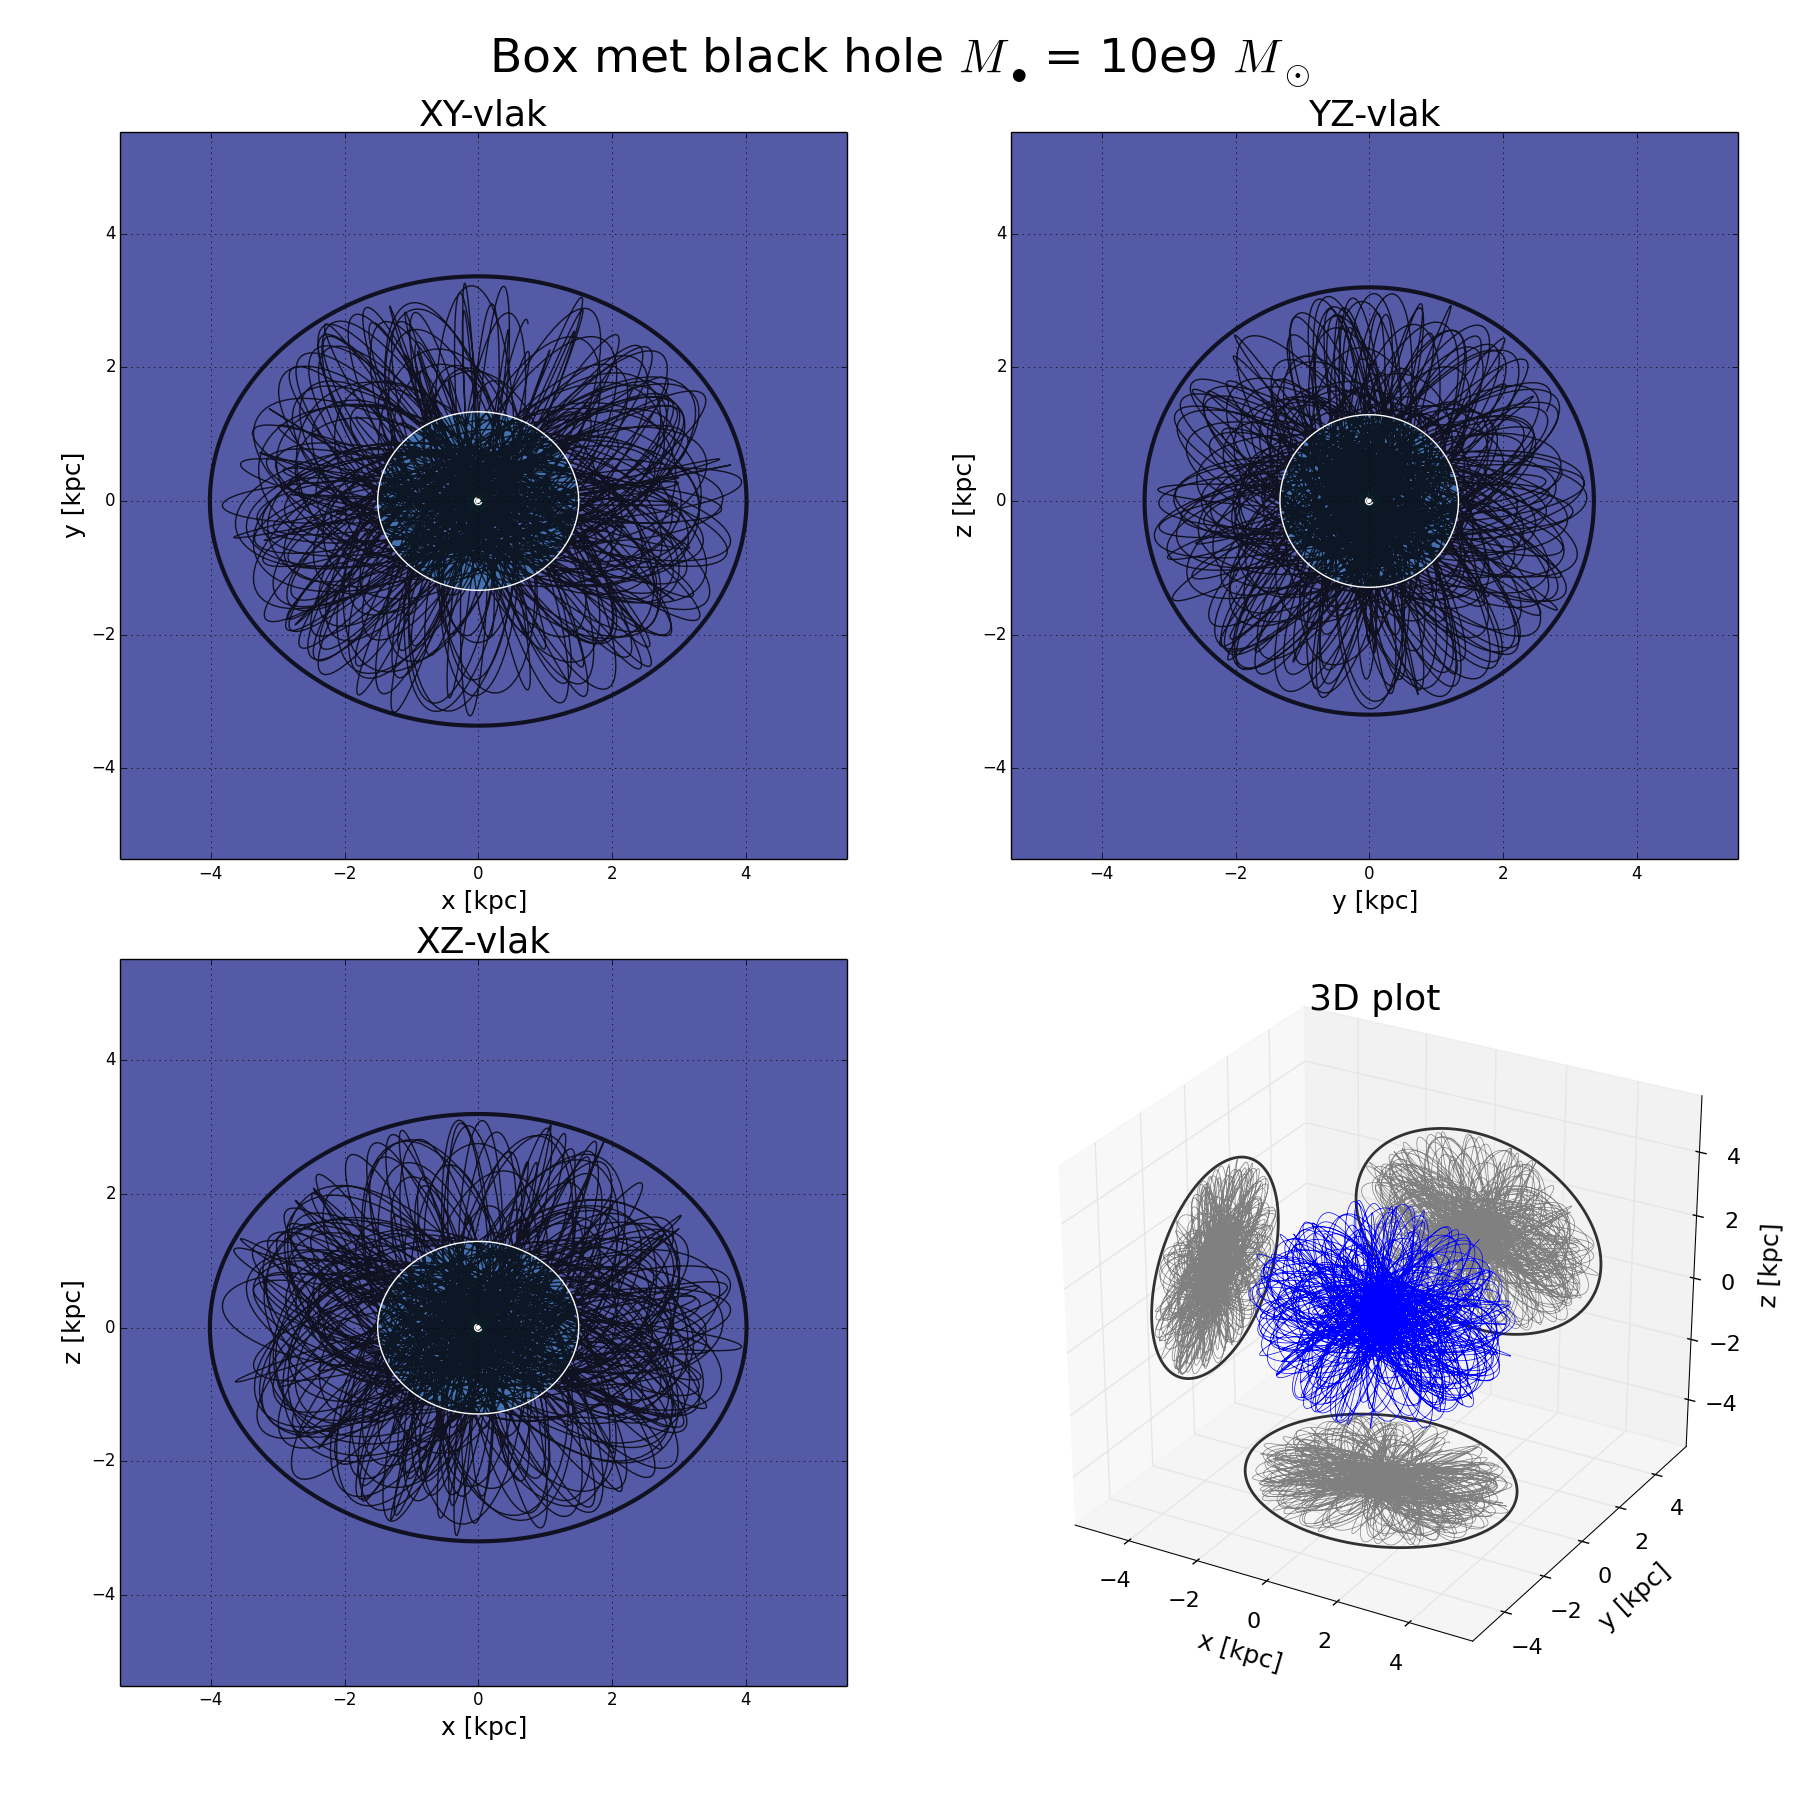
\includegraphics[width=1\textwidth]{img/bh.png}
\caption{Effect van een zeer massief zwart gat}
\label{fig:bigbhplot}
\end{figure}
\vfill

\end{document}